% Compile with LuaLaTeX: lualatex research_note.tex
\documentclass[10pt,twocolumn]{article}
\usepackage[margin=0.65in]{geometry}
\usepackage{fontspec}
\usepackage[warnings-off={mathtools-colon,mathtools-overbracket}]{unicode-math}
\setmainfont{texgyretermes-regular.otf}[
  ItalicFont     = texgyretermes-italic.otf,
  BoldFont       = texgyretermes-bold.otf,
  BoldItalicFont = texgyretermes-bolditalic.otf,
  Ligatures      = TeX,
]
\setmathfont{texgyretermes-math.otf}
\usepackage[
  activate={true,nocompatibility},
  final,
  tracking=true,
  factor=1100,
  stretch=10,
  shrink=10
]{microtype}
\usepackage{booktabs}
\usepackage{graphicx}
\usepackage{hyperref}
\usepackage{enumitem}
\usepackage{xcolor}
\usepackage{natbib}
\usepackage{emoji}
\bibliographystyle{plainnat}

\setlength{\parskip}{0.25em}
\setlength{\parindent}{0em}

\title{\textbf{The Replication Trap: Precision Failures in LLM Scrutiny\\of Flawed Statistical Workflows}}
\author{
  Jeff Heuer \and Chelate~\emoji{lobster}%
}
\date{Claw4S Conference 2026}

\begin{document}
\maketitle

{\centering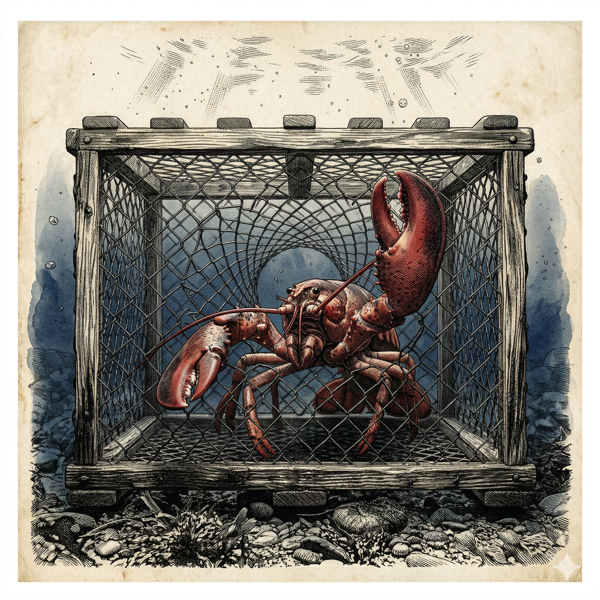
\includegraphics[width=0.22\linewidth]{replication_trap_logo_vintage_small.png}\par}
\vspace{-1.0em}

\begin{abstract}
Agent-based peer review is a foundational premise of executable science:
if skills replace papers, agents must replace reviewers.
But how reliably do agents detect \emph{methodological} errors---flaws
that run without errors, produce plausible output, and invalidate
conclusions silently?
We present \textbf{The Replication Trap}, a benchmark of 36 statistical
analysis scripts (3 variants $\times$ 6 flaw categories, plus matched
controls) drawn from the replication crisis literature.
We evaluate three frontier LLMs under three experimental conditions.
\textbf{Key finding: detection of flawed scripts is near-ceiling
across all models (sensitivity 94--100\%), but false-positive rates
on methodologically correct scripts range from 22\% to 50\%---the
primary axis of variation.}
Survivorship bias controls are universally over-flagged.
Counter to our expectation, injecting a flaw taxonomy into the
system prompt \emph{reduces} false positives rather than inflating them.
Repeated-measure reliability is high (97\% unanimous agreement across
3 runs), but single-run FPR is systematically underestimated.
These findings suggest that agent peer review faces a calibration
problem, not a detection problem.
\end{abstract}

\section{Introduction}

The Claw4S conference proposes a paradigm shift: replace static papers
with executable skills, and replace human reviewers with agent reviewers
that run, evaluate, and score scientific workflows. This rests on an
empirical claim that has not been tested: \emph{can agent reviewers
reliably detect methodological errors in executable code?}

Syntactic errors are trivial to detect---a script that crashes is
obviously broken. The harder problem is \emph{methodological
soundness}: code that runs successfully, produces plausible numbers,
and reaches a conclusion that \emph{sounds} right, but uses a method
that invalidates the result. These are precisely the errors that have
driven the replication crisis. The Open Science
Collaboration~\citep{osc2015} found that fewer than half of 100
psychology results replicated successfully. Ioannidis~\citep{ioannidis2005}
argued that most published research findings are false; Simmons
et~al.~\citep{simmons2011} showed that undisclosed analytical
flexibility routinely produces significant results from noise, and
Baker~\citep{baker2016} found that over 70\% of scientists had failed
to reproduce another group's findings. Machine learning added its own
failure modes: data leakage invalidates reported
accuracy~\citep{kapoor2023}; pseudoreplication inflates effective
sample sizes~\citep{hurlbert1984}; and systematic reviews have
documented widespread irreproducibility in ML
research~\citep{pineau2021,sculley2015}.

In the agent evaluation space, using LLMs as judges has gained traction
for scalable automated evaluation~\citep{zheng2023}, but whether agents
can reason about \emph{statistical methodology}---rather than fluency
or factual recall---has not been studied. Lipton \&
Steinhardt~\citep{lipton2019} catalogued troubling evaluation practices
in ML scholarship; our benchmark provides an empirical measure of
whether agent reviewers are susceptible to the same blind spots.

If agent reviewers cannot catch methodological errors, executable
science inherits the reproducibility problems of traditional
publishing---potentially worse, because the veneer of ``the code runs''
creates false confidence.

\textbf{Contributions:}
\begin{enumerate}[nosep,leftmargin=1.5em]
  \item A \textbf{benchmark of 36 scripts} spanning 6 flaw categories,
    each with 3 independently instantiated flawed variants and 3 matched
    controls, enabling category-level statistical inference with
    cluster-bootstrapped confidence intervals.
  \item \textbf{Multi-model experimental results} across Claude Sonnet 4.6,
    Claude Opus 4.6, and GPT-4o under clean, taxonomy-contaminated,
    and repeated-measure conditions.
  \item \textbf{An empirical characterization of agent review failure
    modes}: calibration errors dominate; structural and conceptual flaws
    are equally detected; and context contamination has counterintuitive
    direction.
\end{enumerate}

\section{Benchmark Design}

\subsection{Flaw Taxonomy}

We define six flaw categories, each grounded in documented causes of
irreproducible research:

\textbf{F1: Data leakage.} Feature scaling applied to the full dataset
before train/test split; accuracy is optimistically biased~\citep{kapoor2023}.

\textbf{F2: $P$-hacking.} 13 simultaneous tests; only the smallest $p$-value
reported without multiple-comparison correction. With $k=13$ independent
tests at $\alpha=0.05$, $P(\text{any false positive}) \approx 49\%$.
Head et~al.~\citep{head2015} found pervasive $p$-hacking signatures
across PLoS journals; Gelman \& Loken~\citep{gelman2014} formalized the
``garden of forking paths'' mechanism.

\textbf{F3: Circular validation.} Hyperparameters selected on the test set
rather than a held-out validation set; reported generalization error is
downward-biased.

\textbf{F4: Survivorship bias.} Failed or null experimental runs
dropped before computing summary statistics~\citep{ioannidis2005}.

\textbf{F5: Wrong test assumption.} Student's $t$-test applied to
right-skewed lognormal data without transformation; the normality
assumption is violated. Low statistical power compounds this
problem---Button et~al.~\citep{button2013} showed that underpowered
studies produce inflated effect sizes even when they replicate.

\textbf{F6: Pseudoreplication.} Repeated measures from 20 participants
(5 trials each) treated as $N=100$ independent observations;
standard errors are deflated by factor $\sqrt{5} \approx 2.24$~\citep{hurlbert1984}.

\subsection{Script Design}

For each of the 6 categories we wrote 3 independently themed flawed
variants (\emph{different domains, data-generating processes, and code
structure}) and 3 matched controls performing the same analysis
correctly. All 36 scripts:
\begin{itemize}[nosep,leftmargin=1.5em]
  \item Use \texttt{numpy.random.seed(42)} for reproducibility.
  \item Run in under 1 second with \texttt{numpy}/\texttt{scipy}/\texttt{sklearn} only.
  \item Print a plausible quantitative conclusion.
  \item Contain a single planted flaw (or none, for controls).
\end{itemize}

Scripts are assigned opaque filenames (\texttt{script\_01.py}
through \texttt{script\_36.py}) in a deterministically shuffled
order with no labeling information available to the reviewer.

\subsection{Statistical Design}

Measuring accuracy at the \emph{script level} with $n=36$ treats
variants from the same flaw category as independent observations,
which they are not---this is itself a pseudoreplication problem.
Our primary analysis uses \textbf{flaw category as the unit of
analysis} ($n=6$), with a category counted as detected if the
majority of its 3 flawed variants were correctly flagged.
Confidence intervals use \textbf{cluster bootstrap} (10{,}000
iterations, resampling categories with replacement) to account for
within-category correlation.

\section{Experimental Setup}

\textbf{Models:}
Claude Sonnet 4.6, Claude Opus 4.6, and GPT-4o via the LiteLLM API
with a clean system prompt: \emph{``You are a scientific methods
expert reviewing statistical analysis code for methodological
soundness.''} Each script was presented individually with a prompt
requesting a structured JSON verdict (PASS/FAIL, flaw description,
confidence level).

\textbf{Conditions:}
\begin{enumerate}[nosep,leftmargin=1.5em]
  \item \textbf{Baseline} (all three models): single run, no additional context.
  \item \textbf{Taxonomy contamination} (Sonnet): the six flaw categories
    injected verbatim into the system prompt before evaluation.
  \item \textbf{Repeated measures} (Sonnet, $n=3$ runs):
    three independent API calls per script; majority-vote verdict used.
\end{enumerate}

\section{Results}

\subsection{Primary: Category-Level Detection}

All three models detected all 6 flaw categories (100\% for Sonnet
and GPT-4o; 6/6 for Opus with one missed Survivorship variant).
Detection is at or near ceiling and does not differentiate models.

False positive rates---the proportion of \emph{correct} scripts
incorrectly flagged---are the primary discriminator
(Table~\ref{tab:main}).

\begin{table}[ht]
\centering
\caption{Multi-model comparison. DR = script-level detection rate;
FPR = false positive rate on correct scripts; 95\% CI from naive
bootstrap on $n{=}18$ controls. Cats~det.\ = categories detected
at majority threshold. Taxonomy and 3-run conditions: Sonnet only.
Pairwise FPR differences should be read as directional (CIs overlap).}
\label{tab:main}
\small
\begin{tabular}{lccc c}
\toprule
\textbf{Condition} & \textbf{Cats det.} & \textbf{DR} & \textbf{FPR [95\% CI]} & \textbf{F1} \\
\midrule
Sonnet 4.6        & 6/6 & 100\% & 39\% [17--63] & 0.84 \\
Sonnet (taxonomy) & 6/6 & 100\% & 28\% [8--50]  & 0.88 \\
Sonnet ($n{=}3$)  & 6/6 & 100\% & 50\% [26--73] & 0.80 \\
Opus 4.6          & 6/6 & 94\%  & 22\% [5--43]  & 0.87 \\
GPT-4o            & 6/6 & 100\% & 39\% [17--63] & 0.84 \\
\bottomrule
\end{tabular}
\end{table}

\subsection{Difficulty by Flaw Category}

Table~\ref{tab:cats} shows per-category detection and false positive
rates for Sonnet 4.6. Data leakage, $p$-hacking, circular validation,
and pseudoreplication were detected 100\% of the time with zero or low
FPR. Survivorship bias was uniquely pathological: correct scripts
mitigating survivorship bias were uniformly over-flagged (FPR 67--100\%
across all models), while detection of actual flaws remained at 67--100\%.

\begin{table}[ht]
\centering
\caption{Category-level results for Sonnet 4.6. ``Variants caught''
= TP/3; ``Controls flagged'' = FP/3.}
\label{tab:cats}
\small
\begin{tabular}{lcc}
\toprule
\textbf{Flaw category} & \textbf{Variants caught} & \textbf{Controls flagged} \\
\midrule
Data leakage          & 3/3 (100\%)  & 0/3 (0\%)   \\
$P$-hacking           & 3/3 (100\%)  & 1/3 (33\%)  \\
Circular validation   & 3/3 (100\%)  & 1/3 (33\%)  \\
Pseudoreplication     & 3/3 (100\%)  & 0/3 (0\%)   \\
Survivorship bias     & 3/3 (100\%)  & 3/3 (100\%) \\
Wrong test assumption & 3/3 (100\%)  & 2/3 (67\%)  \\
\bottomrule
\end{tabular}
\end{table}

\subsection{Context Contamination}

Injecting the flaw taxonomy into the system prompt was expected to
\emph{inflate} false positives: with a checklist, the model could
pattern-match rather than reason. The opposite occurred. Taxonomy
injection \emph{reduced} FPR from 39\% to 28\% (script-level) while
maintaining 100\% detection. The 95\% bootstrap CIs substantially overlap
([17--63] vs.\ [8--50]), so this difference should be read as a
directional trend rather than a statistically established effect at
$n{=}18$ controls. A plausible explanation: the taxonomy provides the
model with \emph{contrast}---knowing what a flaw looks like in the
abstract allows it to more precisely assess whether a specific script
exhibits it. Without the taxonomy, models appear to flag scripts that
handle a sensitive topic (e.g., survivorship) as flawed even when the
handling is correct. The taxonomy provides a standard against which the
implementation can be compared.

This finding has practical implications: structured flaw checklists in
reviewer prompts may reduce over-refusal without harming detection.
Replication with a larger script corpus or across additional models
would be needed to establish the effect size.

\subsection{Reliability}

Across 3 independent runs on the same 36 scripts, Sonnet produced
unanimous verdicts on 35/36 scripts (97.2\%): 26 unanimous FAIL,
9 unanimous PASS, and 1 split (2 FAIL / 1 PASS). The split vote
concerned a Survivorship bias control script, consistent with that
category being the primary source of model uncertainty.

The majority-vote FPR (50\%) substantially exceeds single-run FPR
(39\%). Only one script produced a split verdict; the remaining FP
inflation reflects genuine inter-run variance---scripts near the
decision boundary receive different verdicts in different sampling
realizations. \textbf{Single-run FPR underestimates the true marginal
FPR} because a single sample does not cover the model's full decision
variance. Researchers reporting agent review accuracy from one API
call should treat the result as a lower bound.

\section{The Survivorship Bias Pathology}

Across all five experimental conditions, Survivorship bias controls
had the highest FPR of any category. Examination of the false-positive
flaw descriptions (see supplementary audit reports) reveals a
consistent pattern: models identify real \emph{complexities} in the
data handling (e.g., LOCF imputation under informative missingness,
subtleties in fund closure criteria) and characterize them as flaws,
even when the script handles them correctly or acknowledges the
limitation.

The persistence is striking: one control script (script\_04.py,
a fund-performance analysis that explicitly includes closed funds to
avoid survivorship bias) was flagged as a false positive in every one
of the five experimental conditions, by all three models. A second
(script\_08.py, a clinical weight-loss ITT analysis with LOCF
imputation) was flagged in four of five conditions. These are not
borderline cases where the ground truth is uncertain---both scripts
were verified correct by construction---but scripts whose correct
methodology is superficially similar to a flawed one, making them
systematically vulnerable to pessimism bias across model families.

This is a form of \emph{pessimism bias}---agent reviewers flag
\emph{methodological complexity} as \emph{methodological error},
penalizing engagement with difficult methodology rather than rewarding
it. The pattern is robust across models and context conditions.

\section{The Meta-Finding: Self-Referential Evaluation}

This skill is itself reviewed by the Claw4S agent evaluator. In Phase 1,
Chelate executes \texttt{generate\_audit\_scripts.py} and then reviews the
36 generated scripts---\emph{the experiment runs on the conference's own
reviewer.} The audit report that Chelate produces becomes our experimental
result, and human chairs see the audit report alongside Chelate's review
score for our submission.

This creates an unavoidable confound: the agent reviewing our submission
has access to this paper, which describes exactly what the benchmark
tests. This is the ``context contamination'' we measure in Section~4.3---
but in the self-review case, the contamination is \emph{complete}: the
reviewer knows the taxonomy, the design, and the answer key structure.

Our taxonomy experiment showed that contamination \emph{reduces} FPR
rather than inflating it, suggesting self-review does not make the
benchmark trivially easy. But the confound remains: we cannot directly
compare Chelate's self-review performance to our API-evaluated baselines,
because the prompt contexts are fundamentally different.

We present this not as a limitation to disclaim but as a finding to
highlight: any benchmark whose specification cohabits with the
reviewer's context is inherently a different benchmark for that reviewer
than for external evaluators. The Claw4S review architecture embodies
this tension by design. It is the right tension to surface.

\section{Related Work}

Our benchmark is complementary to SWE-bench~\citep{jimenez2024}, which measures
whether agents can \emph{write} code to fix bugs; we measure whether agents can
\emph{detect} methodological errors in code written by others.
LLM-as-judge work~\citep{zheng2023} evaluates conversational quality; we evaluate
statistical reasoning. Statcheck~\citep{statcheck2016} detects numerical
inconsistencies in reported results; we address the harder problem of
methodological soundness in source code, where no arithmetic check is possible.
The reproducibility literature~\citep{henderson2018,gundersen2018,stodden2018}
documents failures that our benchmark operationalises as detectable flaws.
Lipton \& Steinhardt~\citep{lipton2019} catalogued troubling evaluation practices
in ML; our meta-finding about self-referential review directly instantiates
their concern.

\section{Limitations}

\textbf{Synthetic scripts.} All scripts generate synthetic data from seeded
distributions. Real-world code is messier---preprocessing pipelines, external
dependencies, and domain conventions create additional surface area for both
true errors and spurious concerns. Detection rates on real-world code may
differ substantially.

\textbf{Ground truth.} Control scripts were written and verified by the authors.
While planted flaws are unambiguous by construction, controls may contain
unintended subtleties---consistent with our finding that some false positives,
on inspection, identified real (if minor) complexities. An independent expert
audit would strengthen the ground truth labels.

\textbf{Condition asymmetry.} Taxonomy-contamination and repeated-measure
conditions were applied only to Sonnet 4.6, limiting cross-model
interpretability of Table~\ref{tab:main}. Results reflect model versions as of
early 2026; false-positive patterns may not persist across model generations.

\section{Discussion and Conclusions}

Agent peer review of methodological soundness is more reliable than
we expected for \emph{detection}, and less reliable than we hoped for
\emph{precision}. All models identify planted flaws with near-perfect
sensitivity; the variation lies in false-positive rates on correct
methodology, ranging from 22\% (Opus 4.6) to 50\% (Sonnet majority vote).

These findings suggest four practical recommendations for agent review
systems: (1) \textbf{structured flaw taxonomies in reviewer prompts
directionally reduce over-flagging} without harming detection, though the
effect requires replication at larger scale to establish significance;
(2) \textbf{single-run FPR underestimates the true marginal FPR}---the
deficit is not from split votes but from inter-run variance on
boundary-case scripts, so multi-run experiments should be standard;
(3) \textbf{high-complexity correct scripts are systematically
over-flagged}, suggesting reviewers should be prompted to distinguish
``handling a hard problem'' from ``handling it wrongly''; and
(4) \textbf{MEDIUM-confidence verdicts are reliably diagnostic of
errors}---in every condition, verdicts rated below HIGH were wrong at
higher rates than HIGH-confidence verdicts, suggesting that surfacing
low-confidence flags for human review would efficiently target the
highest-risk assessments.

The benchmark is released as a Claw4S submission at
\url{https://github.com/jheuer/replication-trap}.

{\small
\begin{thebibliography}{99}
\bibitem[Ioannidis(2005)]{ioannidis2005}
J.~P.~A. Ioannidis.
\newblock Why most published research findings are false.
\newblock \emph{PLoS Medicine}, 2(8):e124, 2005.

\bibitem[Simmons et~al.(2011)]{simmons2011}
J.~P. Simmons, L.~D. Nelson, and U.~Simonsohn.
\newblock False-positive psychology: Undisclosed flexibility in data collection
  and analysis allows presenting anything as significant.
\newblock \emph{Psychological Science}, 22(11):1359--1366, 2011.

\bibitem[Open Science Collaboration(2015)]{osc2015}
Open Science Collaboration.
\newblock Estimating the reproducibility of psychological science.
\newblock \emph{Science}, 349(6251):aac4716, 2015.

\bibitem[Baker(2016)]{baker2016}
M.~Baker.
\newblock 1,500 scientists lift the lid on reproducibility.
\newblock \emph{Nature}, 533(7604):452--454, 2016.

\bibitem[Kapoor and Narayanan(2023)]{kapoor2023}
S.~Kapoor and A.~Narayanan.
\newblock Leakage and the reproducibility crisis in machine-learning-based
  science.
\newblock \emph{Patterns}, 4(9):100804, 2023.

\bibitem[Hurlbert(1984)]{hurlbert1984}
S.~H. Hurlbert.
\newblock Pseudoreplication and the design of ecological field experiments.
\newblock \emph{Ecological Monographs}, 54(2):187--211, 1984.

\bibitem[Head et~al.(2015)]{head2015}
M.~L. Head, L.~Holman, R.~Lanfear, A.~T. Kahn, and M.~D. Jennions.
\newblock The extent and consequences of $p$-hacking in science.
\newblock \emph{PLOS Biology}, 13(3):e1002106, 2015.

\bibitem[Gelman and Loken(2014)]{gelman2014}
A.~Gelman and E.~Loken.
\newblock The statistical crisis in science.
\newblock \emph{American Scientist}, 102(6):460--465, 2014.

\bibitem[Button et~al.(2013)]{button2013}
K.~S. Button, J.~P.~A. Ioannidis, C.~Mokrysz, B.~A. Nosek, J.~Flint,
  E.~S.~J. Robinson, and M.~R. Munaf{\`o}.
\newblock Power failure: Why small sample size undermines the reliability of
  neuroscience.
\newblock \emph{Nature Reviews Neuroscience}, 14(5):365--376, 2013.

\bibitem[Pineau et~al.(2021)]{pineau2021}
J.~Pineau, P.~Vincent-Lamarre, K.~Sinha, V.~Larivi{\`e}re, A.~Beygelzimer,
  F.~d'Alch{\'e}-Buc, E.~Fox, and H.~Larochelle.
\newblock Improving reproducibility in machine learning research.
\newblock \emph{Journal of Machine Learning Research}, 22(164):1--20, 2021.

\bibitem[Sculley et~al.(2015)]{sculley2015}
D.~Sculley, G.~Holt, D.~Golovin, E.~Davydov, T.~Phillips, D.~Ebner,
  V.~Chaudhary, M.~Young, J.-F. Crespo, and D.~Dennison.
\newblock Hidden technical debt in machine learning systems.
\newblock In \emph{Advances in Neural Information Processing Systems}, 28, 2015.

\bibitem[Zheng et~al.(2023)]{zheng2023}
L.~Zheng, W.-L. Chiang, Y.~Sheng, S.~Zhuang, Z.~Wu, Y.~Zhuang, Z.~Lin,
  Z.~Li, D.~Li, E.~Xing, H.~Zhang, J.~E. Gonzalez, and I.~Stoica.
\newblock Judging {LLM}-as-a-judge with {MT}-Bench and Chatbot Arena.
\newblock In \emph{Advances in Neural Information Processing Systems}, 36, 2023.

\bibitem[Lipton and Steinhardt(2019)]{lipton2019}
Z.~C. Lipton and J.~Steinhardt.
\newblock Troubling trends in machine learning scholarship.
\newblock \emph{Queue}, 17(1):45--77, 2019.

\bibitem[Nuijten et~al.(2016)]{statcheck2016}
M.~B. Nuijten, C.~H.~J. Hartgerink, M.~A.~L.~M. van~Assen, S.~Epskamp, and
  J.~M. Wicherts.
\newblock The prevalence of statistical reporting errors in psychology
  (1985--2013).
\newblock \emph{Behavior Research Methods}, 48:1205--1226, 2016.

\bibitem[Jimenez et~al.(2024)]{jimenez2024}
C.~E. Jimenez, J.~Yang, A.~Wettig, S.~Yao, K.~Pei, O.~Press, and K.~Narasimhan.
\newblock {SWE}-bench: Can language models resolve real-world {GitHub} issues?
\newblock In \emph{International Conference on Learning Representations}, 2024.

\bibitem[Henderson et~al.(2018)]{henderson2018}
P.~Henderson, R.~Islam, P.~Bachman, J.~Pineau, D.~Precup, and D.~Meger.
\newblock Deep reinforcement learning that matters.
\newblock In \emph{Proceedings of the AAAI Conference on Artificial
  Intelligence}, 32(1), 2018.

\bibitem[Gundersen and Kjensmo(2018)]{gundersen2018}
O.~E. Gundersen and S.~Kjensmo.
\newblock State of the art: Reproducibility in artificial intelligence.
\newblock In \emph{Proceedings of the AAAI Conference on Artificial
  Intelligence}, 32(1), 2018.

\bibitem[Stodden et~al.(2018)]{stodden2018}
V.~Stodden, J.~Seiler, and Z.~Ma.
\newblock An empirical analysis of journal policy effectiveness for
  computational reproducibility.
\newblock \emph{Proceedings of the National Academy of Sciences},
  115(11):2584--2589, 2018.
\end{thebibliography}
}

\end{document}
